Følgende slutning er givet: \\

\begin{figure}[H]
    \centering
    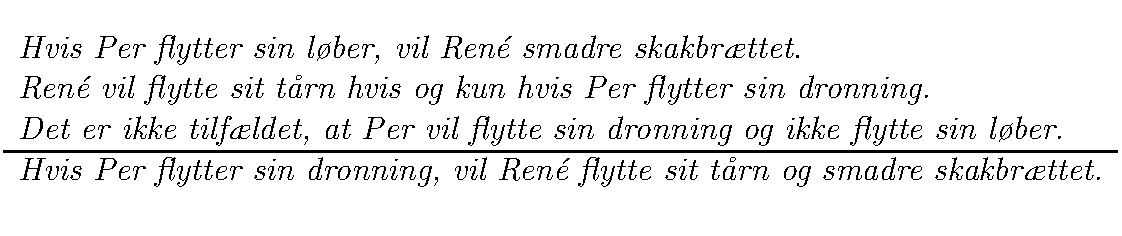
\includegraphics[width=0.9\textwidth]{OpgB/opgaveB.pdf}
    \label{fig:B}
\end{figure}

Først tildeler vi udsagnene nogle prædikatsymboler. \\

$l$: Per flytter sin løber. $s$: René smadrer skakbrættet. $t$: René flytter sit tårn. $d$: Per flytter sin dronning. \\

Herfra kan vi skrive slutninge som: 

\begin{align*}
    &l \rightarrow s \\
    &t \leftrightarrow d \\
    &\neg (d \wedge \neg l) \\
    &\rule{2cm}{0.4pt}\\
    &d \rightarrow (t \wedge s)
\end{align*}

For at slutningen er sand, skal konklusionen være sand antaget at hvert præmis er sandt. Dette kan tjekkes på tableau form:

\begin{figure}[H]
    \centering
    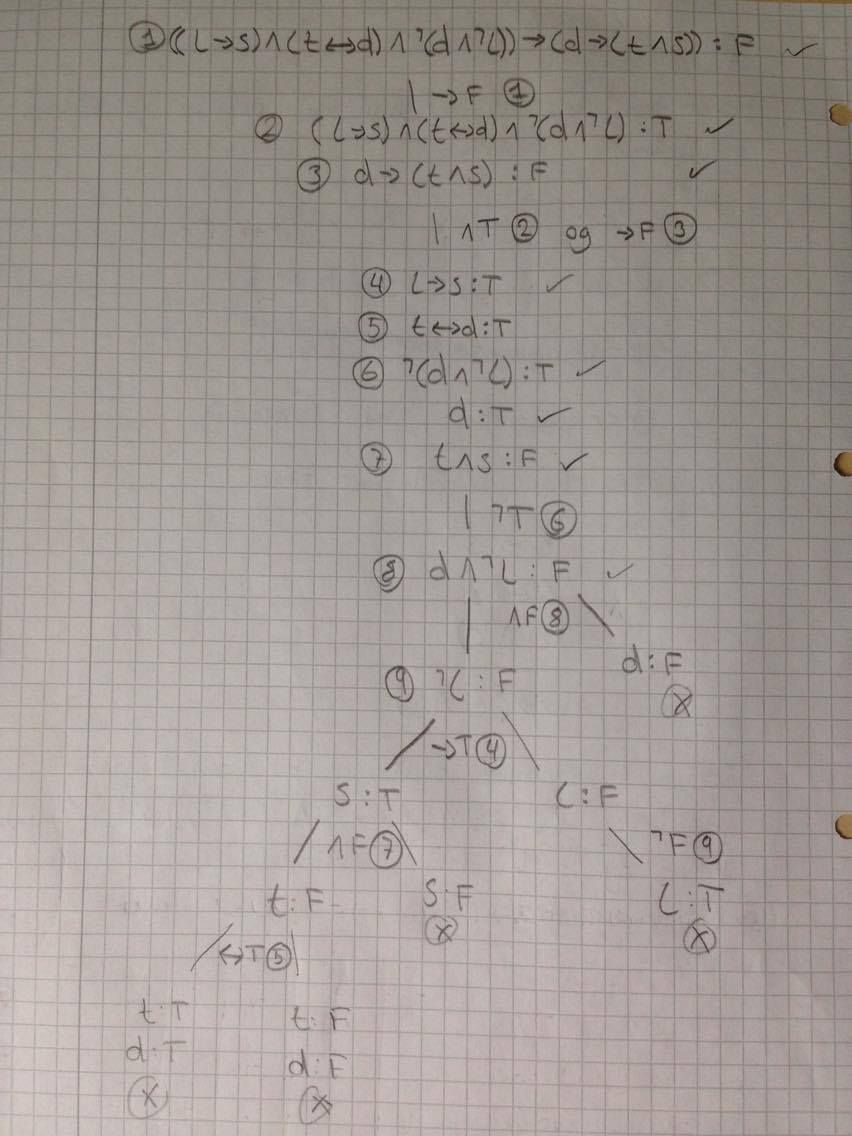
\includegraphics[width=0.8\textwidth]{OpgB/tableauB.jpg}
    \label{fig:B}
\end{figure}

Alle grene er mættede og lukkede svarende til at formlen er gyldig og slutningen er dermed logisk korrekt.